\documentclass[a4paper,12pt]{article}
\usepackage{geometry}
 \geometry{
 a4paper,
 total={170mm,257mm},
 left=20mm,
 top=20mm,
 }
 \usepackage[export]{adjustbox}
\usepackage[english]{babel}
\usepackage[utf8]{inputenc}
\usepackage{fancyhdr}
\usepackage{multicol}
\pagestyle{fancy}
\fancyhf{}
\rhead{\textit{Assignment -2}}
\lhead{\textit{Pul074BEX004}}
\rfoot{\thepage}


\usepackage{mathpazo} % Palatino font
\usepackage{graphicx}
\usepackage{float}


\newcommand{\HRule}{\rule{\linewidth}{0.1mm}} % Defines a new command for horizontal lines, change thickness here
%%%% Anser environment use %%%% Anser environment use %%%% Anser environment use \input{./AnsENV.tex}
%% use \begin{A... {**** argument***}
\RequirePackage{scrextend}

\newenvironment{A}[1]{\textit{Answer:}{\begin{addmargin}[2em]{2em}{#1}\end{addmargin} 
  }}

% just leave some space   
%% use \begin{A... {**** argument***}
\RequirePackage{scrextend}

\newenvironment{A}[1]{\textit{Answer:}{\begin{addmargin}[2em]{2em}{#1}\end{addmargin} 
  }}

% just leave some space   
%% use \begin{A... {**** argument***}
\RequirePackage{scrextend}

\newenvironment{A}[1]{\textit{Answer:}{\begin{addmargin}[2em]{2em}{#1}\end{addmargin} 
  }}

% just leave some space    %% Answer environment 


%%% Question Environment%%%  use 
%%% Question Environment%%%  use 
%%% Question Environment%%%  use \input{./QueENV.tex}   to include
%% Use \begin{Q}....\end{Q}

\newcounter{QC}
\setcounter{QC}{1}
\newenvironment{Q}[1]{
    \section{Question -\arabic{QC}} \stepcounter{QC}{\large\textbf{#1}}
}

%%% Question Environment%%%

   to include
%% Use \begin{Q}....\end{Q}

\newcounter{QC}
\setcounter{QC}{1}
\newenvironment{Q}[1]{
    \section{Question -\arabic{QC}} \stepcounter{QC}{\large\textbf{#1}}
}

%%% Question Environment%%%

   to include
%% Use \begin{Q}....\end{Q}

\newcounter{QC}
\setcounter{QC}{1}
\newenvironment{Q}[1]{
    \section{Question -\arabic{QC}} \stepcounter{QC}{\large\textbf{#1}}
}

%%% Question Environment%%%

 %% Question Environment 


%%%%%% generate table from https://truben.no/table/ and paste bwtween \begin{DT} and end
%% use \input{./diffTable.tex}

\usepackage[table]{xcolor}
\usepackage{array}
\rowcolors{2}{blue!20}{white}
\newcommand{\head}[1]{%
   \textcolor{black}{\textbf{#1}}}
   
\renewcommand{\arraystretch}{1.5}

\setlength{\arrayrulewidth}{0.5mm}
\newenvironment{DT}[2]
{\begin{table}[H]
   \centering
   \sffamily
   \newcommand{\Cap}{\caption{#1 VS #2}}
 \begin{tabular}{|>{\cellcolor{cyan!15}\color{black!100}\bfseries}m{3.5cm}| m{6.5cm}| m{6.5cm}|}
     \rowcolor{cyan!15}
     \hline
     \head{KEYS} & \head{#1} & \head{#2} \\ \hline \hline
    } 
    {
    \hline
  \end{tabular}
  \Cap
\end{table}
} %% Diff table environment 

\begin{document}

%----------------------------------------------------------------------------------------
%	TITLE PAGE
%----------------------------------------------------------------------------------------



\begin{titlepage} % Suppresses displaying the page number on the title page and the subsequent page counts as page 1

	\begin{figure}[H]
	\centering	
	
\includegraphics[scale=0.2]{tulogo.jpg} 
	\end{figure}
	
	\center % Centre everything on the page
	%------------------------------------------------
	%	Headings
	%------------------------------------------------
	
	\textsc{\LARGE Institute of Engineering , Central Campus,Pulchowk}\\[1.5cm] % Main heading such as the name of your university/college
	
	%\textsc{\Large Computer Network}\\[0.5cm] % Major heading such as course name
	
	
	%\textsc{\large ASSIGNMENT  \#2}\\[0.5cm] % Minor heading such as course title+
	
	%------------------------------------------------
	%	Title
	%------------------------------------------------
	
		\HRule\\[0.4cm]
	
	{\huge\bfseries COMPUTER NETWORKS Assignment -2}\\[0.4cm] % Title of your document
	
	\HRule\\[1.5cm]
	
	%------------------------------------------------
	%	Author(s)
	%------------------------------------------------
	\vfill\vfill
	\begin{minipage}{0.4\textwidth}
		\begin{flushleft}
			\large
			\textbf{Submitted BY:} \\
			Amrit Prasad Phuyal\\ % NAME
	Roll: PULL074BEX004 % Roll
		\end{flushleft}
	\end{minipage}
	~
	\begin{minipage}{0.4\textwidth}
		\begin{flushright}
			\large
			\textbf{Submitted To:}\\
			{\normalsize SARAD KUMAR GHIMIRE\\Department of Electronics and Computer Engineering} % Department's Name 
		\end{flushright}
	\end{minipage}
	
	% If you don't want a supervisor, uncomment the two lines below and comment the code above
	%{\large\textit{Author}}\\
	%John \textsc{Smith} % Your name
	
	%------------------------------------------------
	%	Date
	%------------------------------------------------
	
	\vfill\vfill\vfill % Position the date 3/4 down the remaining page
	
	{\large\today} % Date, change the \today to a set date if you want to be precise
	
	%------------------------------------------------
	%	Logo
	%------------------------------------------------
	
	%\vfill\vfill
	%
\includegraphics[width=0.3\textwidth]{tulogo.jpg}\\[0.5cm] % Include a department/university logo - this will require the graphicx package
	 
	%----------------------------------------------------------------------------------------
	
	\vfill % Push the date up 1/4 of the remaining page
	
\end{titlepage}

%----------------------------------------------------------------------------------------
\pagenumbering{gobble}
\tableofcontents
\pagebreak
\listoffigures
\pagebreak
\listoftables
\pagebreak
\pagenumbering{arabic}

%%%%########11111 one
\begin{Q}
{What is guided transmission media? Explain the different guided transmission media with their features.}
\end{Q}

\begin{A}{Guided Transmission media also termed as Bounded Media which uses Physical medium to transfer data. Here signals are directed and contained within the media. They are generally used for Short distance data transfer and are considered fast and secure medium as compared to Unguided media. It includes Twisted-Pair Cable, Coaxial Cable, and Fibre-Optic Cable.
\begin{enumerate}
\item \textbf{Twisted-Pair Cable:}\\ Here the physical medium (Pair of copper cables ) are twisted and covered with protective sheath. it is one of the popular and cheapest medium of data transfer. Twisting is done to reduce the Electromagnetic Interference between the signals. it has frequency range 0-3.5 Khz. It is further divided into:
\begin{figure}[h]
\centering
	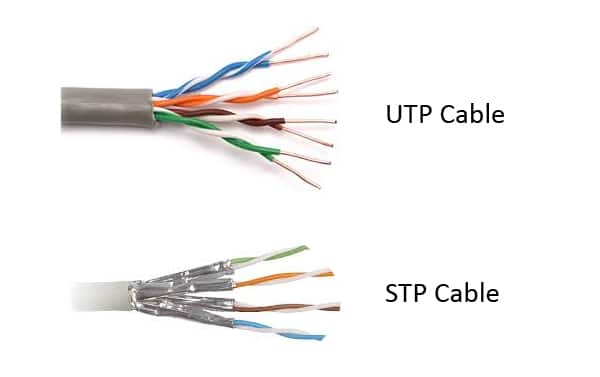
\includegraphics[scale=0.7,cframe=blue 0.5pt 3pt]{utpstp.jpg}
	\caption{{UTP and STP cable}}
\end{figure}
	\begin{enumerate}
   		\item \textbf{Unshielded Twisted Pair Cable (UTP):}\\UTP lacks additional shelding around each pair but they are designed in such a way that the twisting rates almost cancel the interference . These are cheaper ,easier to install,high speed capacity but limited to shorter distance(100m) or LAN.
		\item \textbf{Shielded Twisted Pair Cable (STP):}\\STP has jacket of aluminum or similar metal to block the external interference.It is faster ,safer but is heavy and expensive due to additional coating.
	\end{enumerate}
\item \textbf{ Coaxial Cable}\\
\begin{figure}[h]
\centering
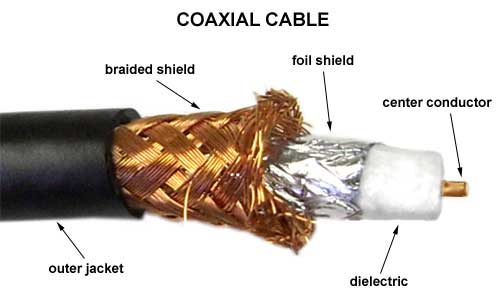
\includegraphics[scale=0.7,cframe=blue 0.5pt 3pt]{coaxcable.jpg} 
\caption{Coaxial Cable}
\end{figure}
Here the conductors are parallel to each other both separated and covered by insulating materials.Center conductor is Copper  surrounded by insulator then by  metallic wrap which acts as shielding  and finally by last insulator jacket.It is more immune to noise and provide higher bandwidth while it is expensive than Twisted pair.
\item \textbf{Fibre-Optic Cable}\\
\begin{figure}[h]
\centering
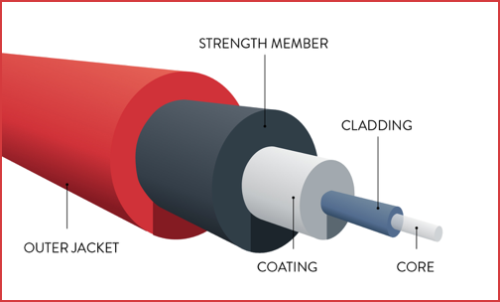
\includegraphics[scale=0.7,cframe=blue 0.5pt 3pt]{Opticalfiber.png} 
\caption{Optical Fiber}
\end{figure}
Optical fiber are made up of glass or plastic and work on the principle of Total internal reflection. Here light is transmitted after being modulated and  receiver demodulate.The Center area Core is the main highway and very narrow. The center part cladding helps lights to be concentric to core and finally jacket acts as insulator.The data transmission is faster and is more immune to environmental and E-M interference. It is light weight, reliable and use in long distance data transmission. the drawbacks are expensive and very difficult to maintain.
\end{enumerate}
}
\end{A}



%%%%222222 TWO

\begin{Q}
{
What is switching? What is the importance of switching in a communication system?}

\end{Q}

\begin{A}{  Switching is the Technique to determine the best route for data from sender to receiver  or between two nodes . It may involves numerous number of intermediate Nodes to handle the data . It includes three types of Switching: Message, Circuit and Packet Switching.
\begin{multicols}{2}
In \textbf{Message switching} each message has its Addressing information appended to it so that it follows the best route to destination. Here no dedicated connection is established so helps to reduce traffic congestion but the message has to be stored in every intermediate nodes.
\columnbreak
\begin{figure}[H]
\centering
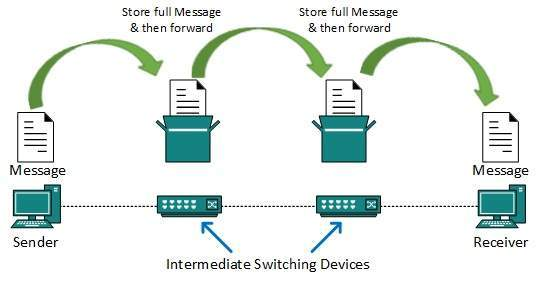
\includegraphics[scale=0.45,cframe=blue 0.5pt 3pt]{message_switching.jpg} 
\caption{Message Switching }
\end{figure}
\end{multicols}
%%
\begin{multicols}{2}
In \textbf{Circuit switching} Dedicated line is used for the whole connection period . The dedicated path between sender and receiver  makes the whole setup reliable while there is high chance of resource wastage. Telephones lines are best examples of Circuit Switching
\columnbreak
\begin{figure}[H]
\centering
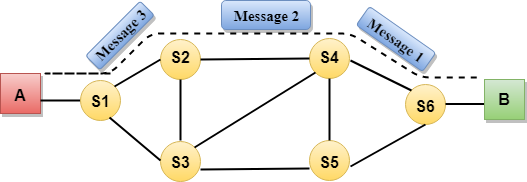
\includegraphics[scale=0.6,cframe=blue 0.5pt 3pt]{circuit-switching.png} 
\caption{Circuit Switching }
\end{figure}
\end{multicols}
%%
\begin{multicols}{2}
In \textbf{Packet Switching} whole data is spited in to smaller chunks called Packets and  sent over network  with source and destination address attached to each message header.Here no dedicate  path is needed as packets travel across networks to destination using the shortest path available, which makes this technique less reliable.
\columnbreak
\begin{figure}[H]
\centering
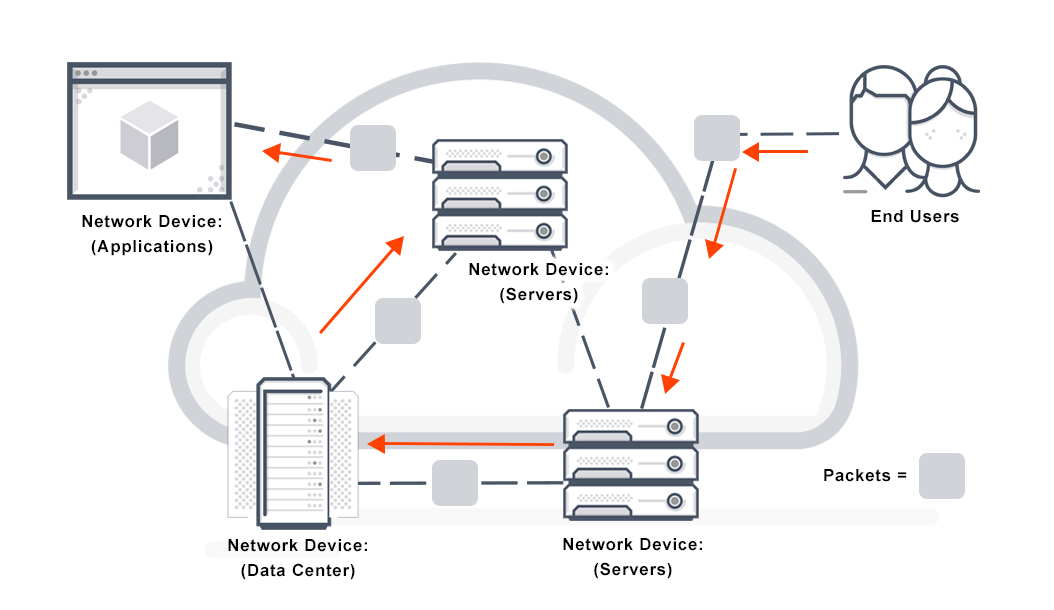
\includegraphics[scale=0.25,cframe=blue 0.5pt 3pt]{packet-switching.png} 
\caption{Packet Switching }
\end{figure}
\end{multicols}
%%
In communication system there are multiple nodes which may be endpoints or redistribution points .In order to communicate between two different nodes , intermediate nodes are essential for data transfer or temporary storage .In this way right data reach the destination accurately and  quickly, the whole process is known as Switching and it is important in Communication.
}
\end{A}

%%%%33333%%%
\begin{Q}
{Discuss briefly on:}
\end{Q}
%%Bandwidth%%
\subsection{Bandwidth:}
\begin{A}
{It is the measurement of the amount of data transmitted over the network  within a certain period. It can be described as the data  capacity of a transmission medium or a network. It is more of a theoretical unit, so is not affected by physical interference and is measured in Bits . To compare with the real world  let's take water as data and tap/pipe as medium, here the speed of water flowing in pipe or coming out of it  is the bandwidth of the tap.}

\end{A}

%%Throughput%%
\subsection{Throughput:}
\begin{A}{
It is a Practical unit for the amount of data  flowing in the network in a certain time or  data received by destination in a given time. It is affected by real world interference and heavily depends on latency. Compared with the real world , it is the amount of water collected from tap output.its measurement units is bits per second.}

\end{A}

%%%Delay%%
\subsection{Delay:}
\begin{A}
{It is the amount of time required for a packet 
to travel from source to destination. In other words it is the processing time of a packet in a network.There are mainly four types of delay in networking.Transmission Delay is the time taken to put a packet in transmission medium by host. Propagation delay  is the time required to transmit a bit from one end of a link to another. Queuing delay is the time spent in a buffer by the packet before being processed.Processing Delay is the time spent to process a particular packet(header) generally by switch or receiver.}

\end{A}

%%%Latency%%
\subsection{Latency:}
\begin{A}
{It is the amount of time required for a packet to travel from one end of a network and emerge at the other end and measured Round Trip Time (RTT).In simple terms it is a measure of delay and it's unit is millisecond(ms).Geography is the major cause for latency , farther the parties higher the latency. Compared with real world it is the amount of time required by water to travel from tank to tap.}

\end{A}

%%%RTT%%
\subsection{RTT:}
\begin{A}
{
Round Trip Time (RTT) also known as Round Trip Delay(RTD). It  is the time in millisecond between  a signal/request   sent and  acknowledged received by the sender. Physical distance , transmission medium and network congestion are some parameters that affect the RTT. Caching and load distribution are some major ways to reduce RTT.}
\end{A}

%%%%ISDN%%%
\subsection{ISDN:}
\begin{A}
{
Integrated Services Digital Network (ISDN) is the communication standard or the technology for transfer of voice and data over digital networks.It had the advantage of faster data transfer or calls and method enable two calls in same telephone lines simultaneously.it has maximum speed of 128 kbit/s. }

\end{A}
%%%%%
%%%%$$$ differentiate between


\begin{Q}
{Differentiate between}
\end{Q}

%%FDM vs. TDM
\subsection{FDM vs. TDM}
\begin{DT}{FDM }{ TDM}
    Full Form           & Frequency Division Multiplexing                                                                                            & Time Division Multiplexing                                                                \\
    Definition          & Multiple data signals are packed together to transfer using shared communication medium through simultaneous transmission. & Incoming data signals are divided as per time division  and transmit over common channel. \\
    Works with          & Only Analog signal                                                                                                         & Both Analog and Digital Signal                                                            \\
    Complexity and Cost & Complex Circuit at both tx,rx  end and Expensive                                                                           & Simple circuit and Cheap                                                                  \\
    Sharing             &  Frequency sharing takes place.                                                                                            & Time sharing takes place.                                                                 \\ 
    Efficiency          & Quite Inefficient                                                                                                          & Efficient                                                                                 \\
    Necessities         & Guard Band( unused part of radio spectrum)                                                                                 &  Synchronization Pulse                                                                    \\
    Propagation Delay   & Very Low                                                                                                                   & As signal are transmitted in different time-slots,propagation delay is high                \\
\end{DT}

%%%%Circuit switching vs. packet switching
\subsection{Circuit switching vs. Packet switching}
\begin{DT}{Circuit Switching }{ Packet Switching}
    Designed for                & Voice Communication                                                                    & Data Transmission                                                                                           \\
    Process                     & Message is received in the order, as sent from the source.                              & Message is received Out of order and later assembled and destination                                        \\
    Connection Types            & Connection Oriented i.e require to setup fixed connection before data begin to transmit & Connection less i.e Packets follows the best possible route so doesn't required dedicated path to be setup. \\
    Processing of Data at       & Data is processed at source system only                                                 & All intermediate nodes( for header)                                                                         \\
    Reliability and Resource    & More reliable,but may cause Resource waste                                              & Less reliable and doesn't use Resource waste                                                                \\
    Transmission Type           & End to End transmission.                                                                & Store and forward transmission.                                                                             \\
    Implementation in OSI model &  At Physical Layer                                                                      & At Network Layer                                                                                            \\
    Bandwidth and Delay         & Fixed                                                                                   & Dynamic                                                                                                     \\
\end{DT}
%%%Datagram vs. virtual circuit switching
\subsection{Datagram vs. Virtual circuit switching}
\begin{DT}{Datagram Switching}{Virtual Circuit Switching }
 Connection Types    & Connectionless as it doesn't require allocation of the buffer, CPU, Bandwidth for data transfer              & Connection-Oriented as those resources are to be reserved before data transfer.             \\
    Process             & The packet is received out of order and assembled at the destination as the packet follows the optimal path. & Packets reach in order to the destination as data follows the same path.                    \\
    Complexity and cost & Easy to setup and maintain and cheaper.                                                                      & Difficult to set up and maintain and expensive due to the requirement to reserve resources. \\
    Header types        & Different headers with information of other data packets  are used.                                          & As the same path followed by all the data packets, a common and same header is used.        \\
    Reliability         & Less reliable than Virtual Circuit switching.                                                                & Very relaible as recources and connection path are dedicated.                               \\
   
\end{DT}

\end{document}
